\documentclass{beamer}

%Russian-specific packages
%--------------------------------------
\usepackage[T2A]{fontenc}
\usepackage[utf8]{inputenc}
\usepackage[russian]{babel}
%--------------------------------------

\usepackage{booktabs}
\usepackage{graphicx}

\title{Оптимизация функции, задаваемой регрессионным лесом}
\author{Влад Ягламунов}
\date{}

\begin{document}

\maketitle

\begin{frame}
    \frametitle{Задача}
    \begin{itemize}
            \item Дано: Обученный регрессионный лес
            \item Найти: Области, где лес возвращает минимальное и максимальное значение
    \end{itemize}
\end{frame}

\begin{frame}
    \frametitle{Последовательная оптимизация основанная на модели Sequential Model-Based Optimization (SMBO)}
    \begin{itemize}
            \item Получаем значения в различных точках 
            \item По ним строиться регрессионная модель
            \item Модель позволяет предсказать минимум оптимизируемой функции
            \item В точках минимума запрашиваем значения
    \end{itemize}
    \vfill
    Sequential Model-based Algorithm configuration (SMAC)
\end{frame}

\begin{frame}
\frametitle{Эвристический алгоритм}
\begin{columns}
    \column{.5\textwidth}
    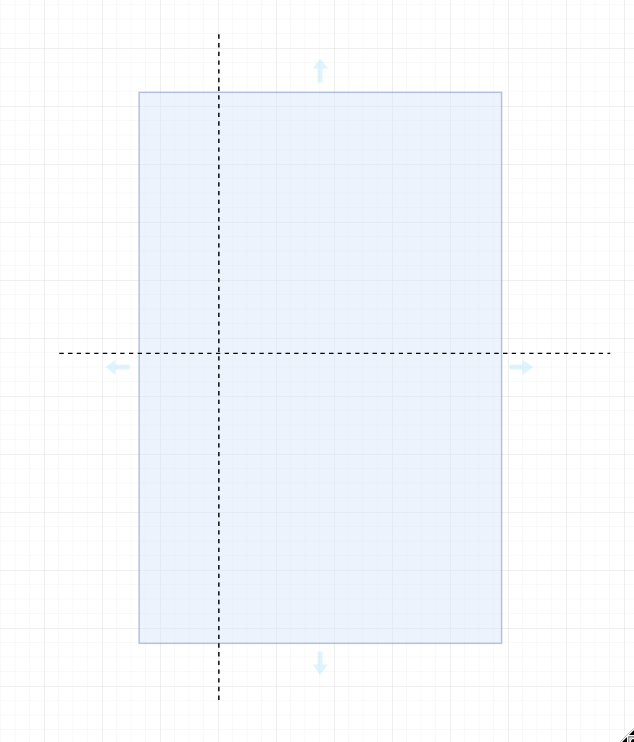
\includegraphics[width=\textwidth]{split.png}
    \column{.5\textwidth}
    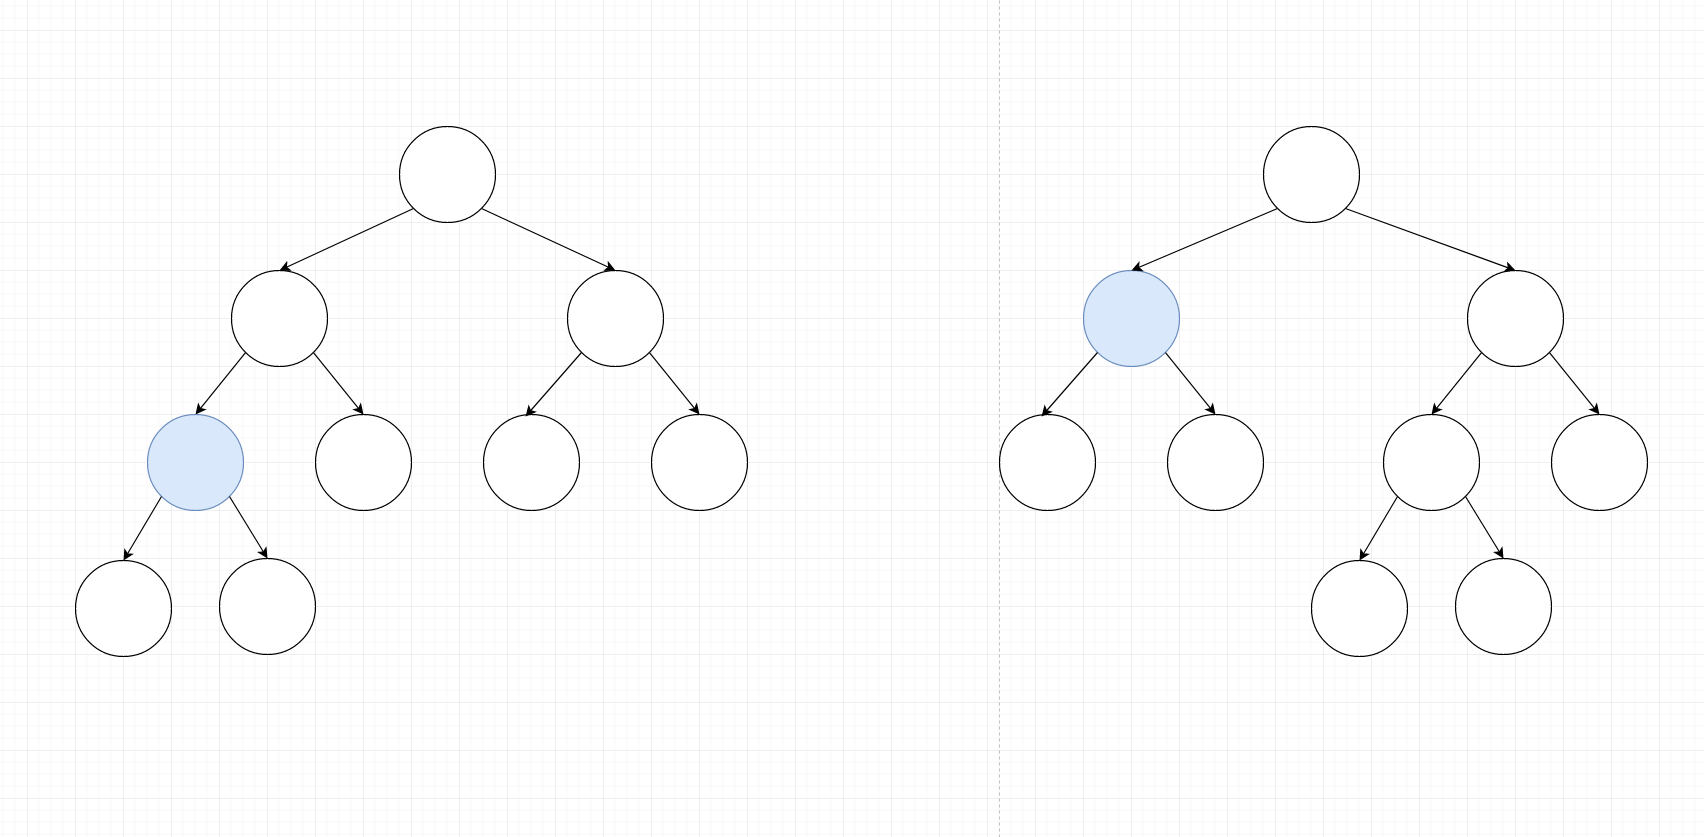
\includegraphics[width=\textwidth]{tree.png}
\end{columns}
    \vfill
    \[
        value[v] = \max(value[v.left], value[v.right])
    \]Эвристика: 
    \[
        i = \arg \max_{v \in trees}(|value[v.left] - value[v.right]|)
    \]
\end{frame}

\begin{frame}
    \frametitle{Эвристический алгоритм (Оптимизация)}
    \begin{center}
    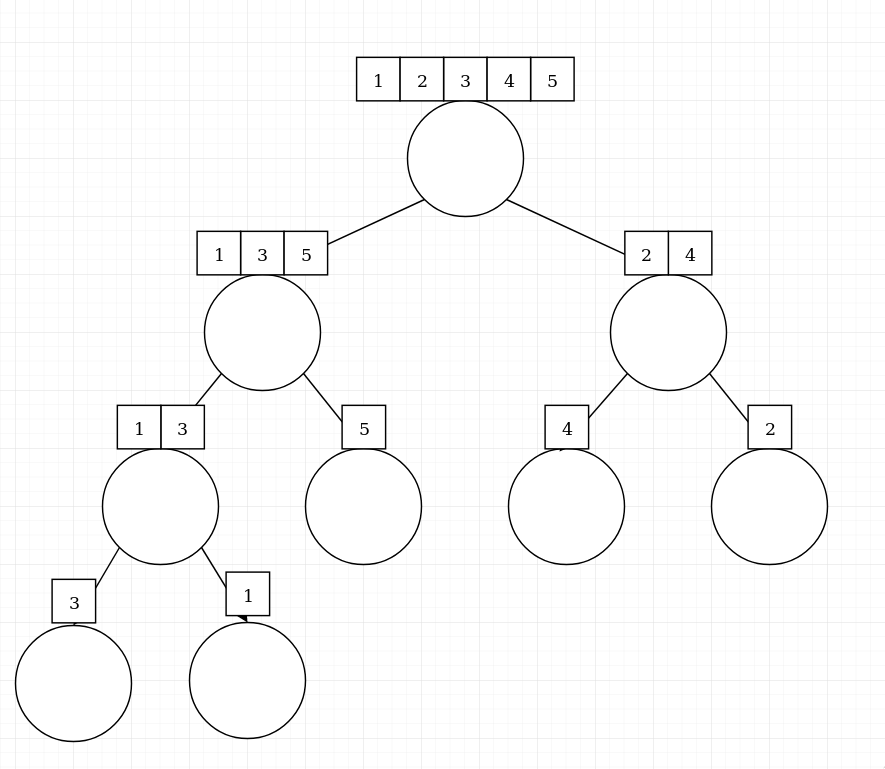
\includegraphics[height=0.8\textheight]{merge.png}
    \end{center}
\end{frame}

\begin{frame}
\frametitle{Алгоритм имитации оджига}
    \begin{center}
    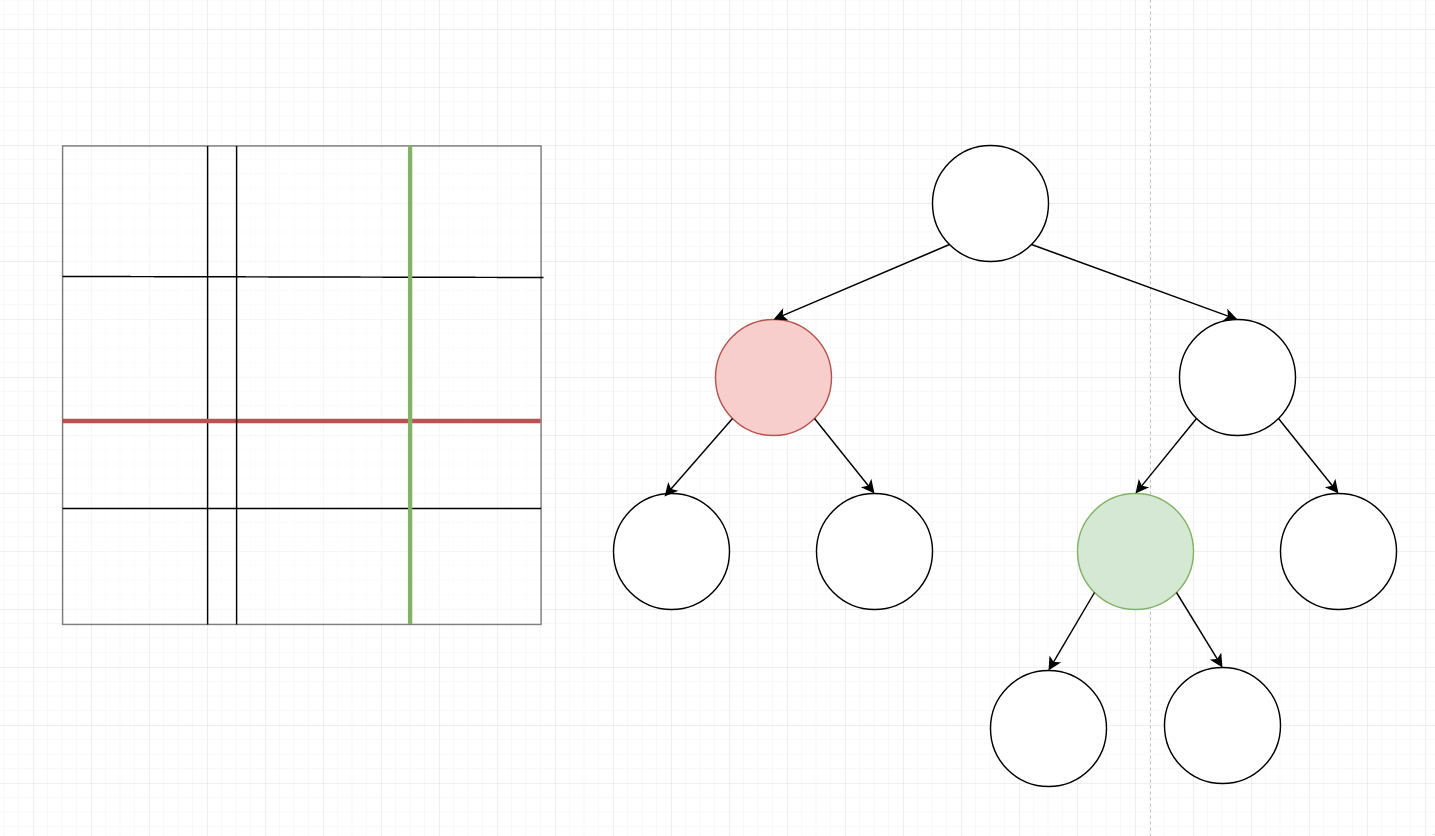
\includegraphics[width=\textwidth]{gena.png}
    \end{center}
\end{frame}

\begin{frame}
\frametitle{Алгоритм имитации оджига}
\begin{columns}
    \column{.5\textwidth}
    Если значение ухудшилось, то переходим с вероятностью 
    \[
    p=\alpha + (1 - \alpha) \frac{i}{N}
    \]
    N --- количество итераций\\
    i --- номер итераций
    \column{.5\textwidth}
    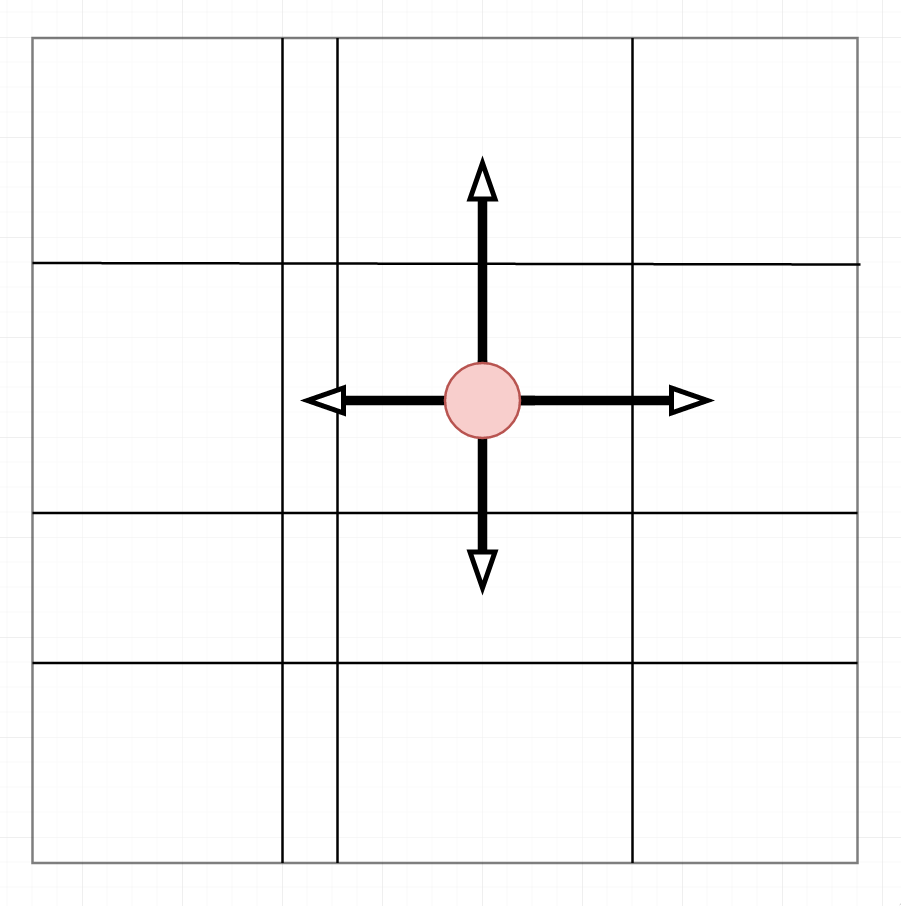
\includegraphics[width=\textwidth]{gena_move.png}
\end{columns}
\end{frame}

\begin{frame}
    \frametitle{Сравниваемые алгоритмы}
    \begin{itemize}
            \item Перебор
            \item Перебор с погрешностью $<5\%$
            \item Рандом
            \item ''Оджиг''
            \item Эвристика
            \item Эвристика с погрешностью $<5\%$
            \item Эвристика с погрешностью $<15\%$
    \end{itemize}
\end{frame}

\begin{frame}
    \frametitle{Использованные данные}
    \begin{center}
        \begin{tabular}{|l|l|l|}

        \hline
         
        название        & элементы  & признаки \\

        \hline

        diabetes        & 442    & 9     \\
        boston          & 506    & 12    \\
        autoPrice       & 159    & 16    \\
        wisconsin       & 194    & 33    \\
        strikes         & 625    & 7     \\
        kin8nm          & 8192   & 9     \\
        house\_8L       & 22784  & 9     \\
        house\_16H      & 22784  & 9     \\
        mtp2            & 274    & 1143  \\

        \hline

    \end{tabular}
    \end{center}
\end{frame}

% \begin{frame}
% \frametitle{Тестирование}
% \hspace*{-0.8cm}
%     \begin{tabular}{l l l l l l l}

%         название        & элементы  & признаки & N & время & N & время \\

%         \toprule

%         diabetes        & 442    & 9     & 30 & 1.07  & 50       & 20\\
%                         &        &       & 30+5\% & 0.24  & 50+5\%      & 5\\
%         boston          & 506    & 12    & 30 & 0.27  & 100      & 1\\
%         autoPrice       & 159    & 16    & 30 & 0.01  & 100      & 6\\
%         wisconsin       & 194    & 33    & 30 & 17    & 30+5\%   & 55\\
%         strikes         & 625    & 7     & 30 & 0.3   & 100      & 1.5\\
%         kin8nm          & 8192   & 9     & 30 & 176   & 30+5\%   & 77\\
%         house\_8L       & 22784  & 9     & 30 & 30    & 30+5\%   & 29\\
%         house\_16H      & 22784  & 9     & 20 & 112   & 20+5\%   & 55\\
%         mtp2            & 274    & 1143  & 30 & 0.30  & 60       & 1.0\\

%     \end{tabular}
% \hspace*{-0.8cm}
% \end{frame}

\begin{frame}
    \frametitle{Тестирование (Время работы)}
    \begin{center}
    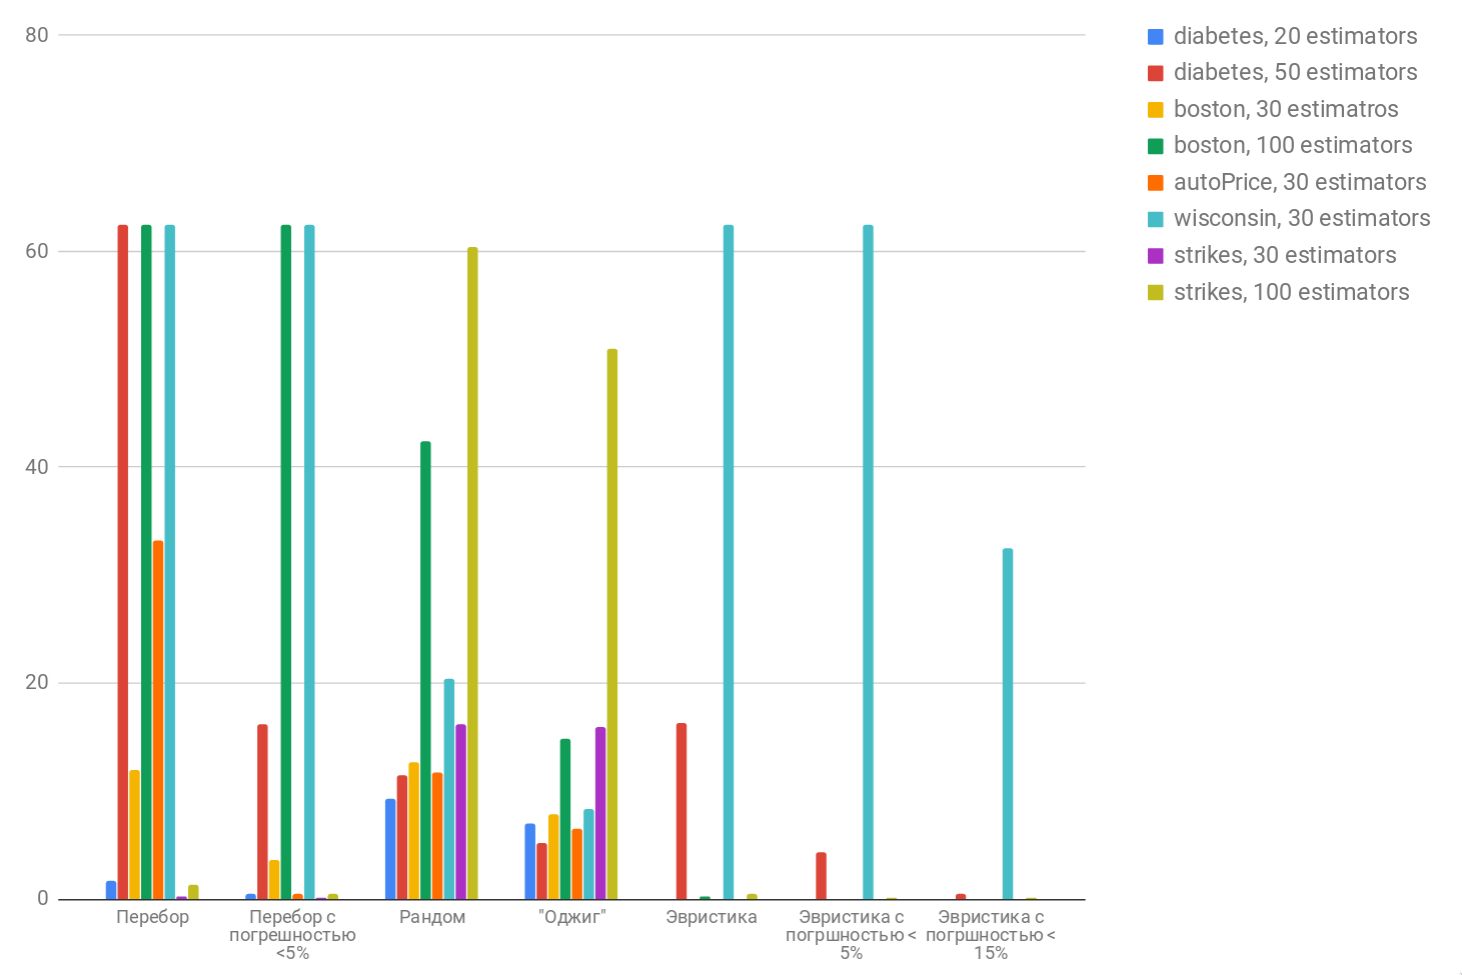
\includegraphics[width=\textwidth]{graph_time1.png}
    \end{center}
\end{frame}

\begin{frame}
    \frametitle{Тестирование (Время работы)}
    \begin{center}
    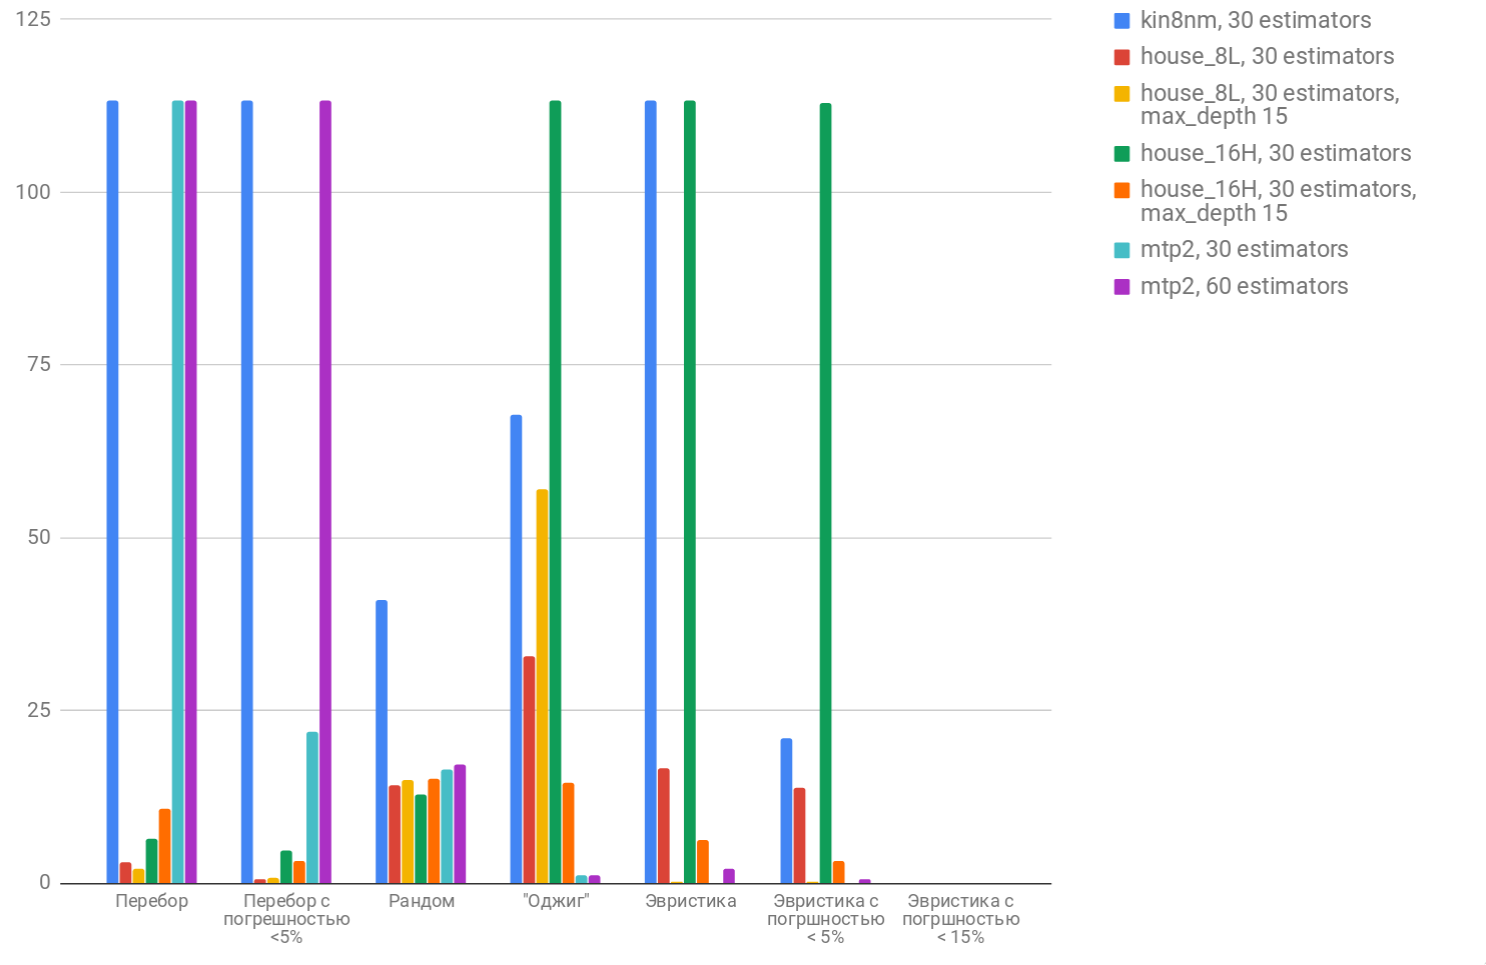
\includegraphics[width=\textwidth]{graph_time2.png}
    \end{center}
\end{frame}

\begin{frame}
    \frametitle{Тестирование (Ошибка)}
    \[
        error = \frac{min - min_{true} + max_{true} - max}{max_{true} - min_{true}}
    \]
    \begin{center}
    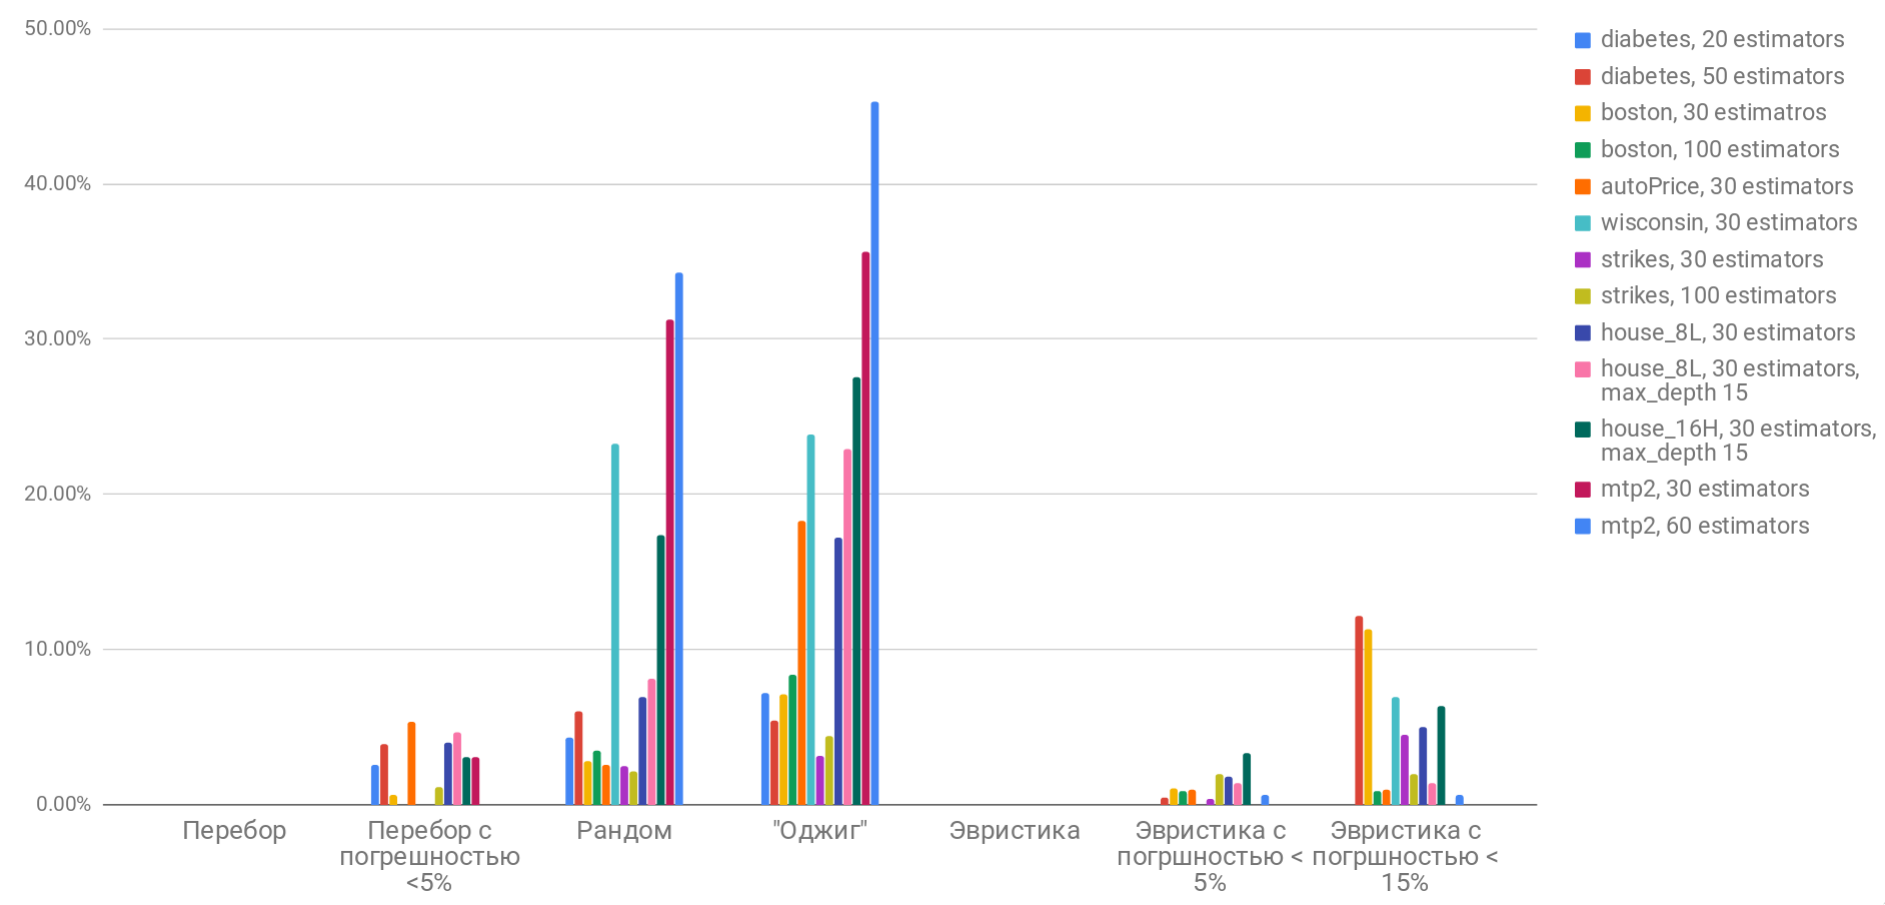
\includegraphics[width=\textwidth]{graph_error.png}
    \end{center}
\end{frame}

\begin{frame}
\frametitle{Визуализация}
    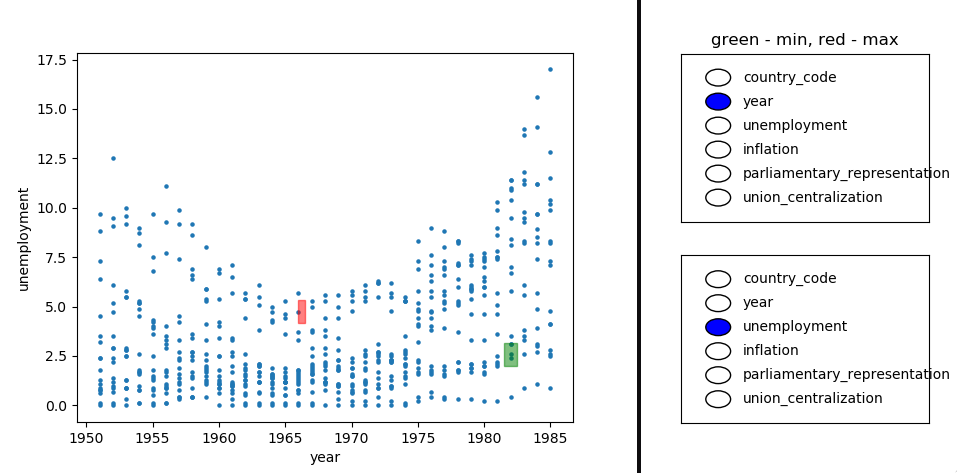
\includegraphics[width=\textwidth]{visual.png}
\end{frame}

\end{document}
